% 2002 年全国旧课程理科第 10 题：函数图象选项
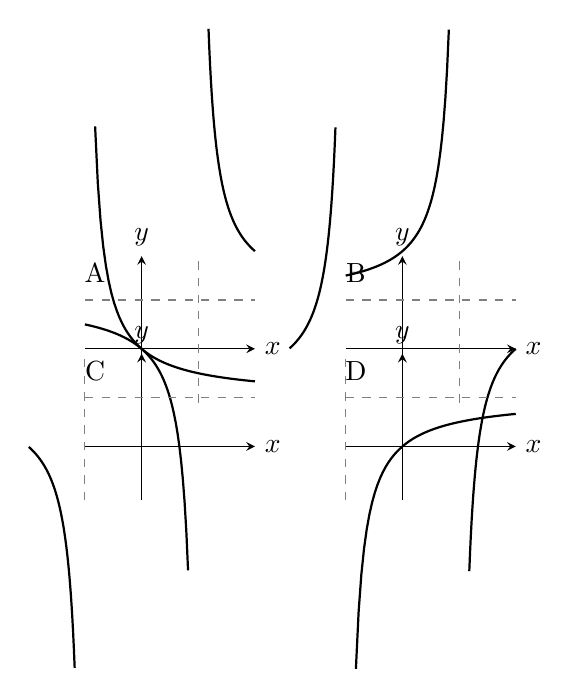
\begin{tikzpicture}[x=0.72cm,y=0.62cm,>=stealth]
  \foreach \sx/\sy/\optlabel in {0/2/A,4.6/2/B,0/0/C,4.6/0/D}
  {
    \begin{scope}[shift={(\sx,\sy)}]
      \draw[->] (-1.0,0)--(2.0,0) node[right] {$x$};
      \draw[->] (0,-1.1)--(0,1.9) node[above] {$y$};
      \node at (-0.82,1.55) {\optlabel};
    \end{scope}
  }
  % A: y=1+1/(x-1)
  \begin{scope}[shift={(0,2)}]
    \draw[dashed,gray] (1,-1.1)--(1,1.9);
    \draw[dashed,gray] (-1,1)--(2,1);
    \draw[thick,domain=-1:0.82,samples=60] plot (\x,{1+1/(\x-1)});
    \draw[thick,domain=1.18:2,samples=60] plot (\x,{1+1/(\x-1)});
  \end{scope}
  % B: y=1-1/(x-1), the correct graph
  \begin{scope}[shift={(4.6,2)}]
    \draw[dashed,gray] (1,-1.1)--(1,1.9);
    \draw[dashed,gray] (-1,1)--(2,1);
    \draw[thick,domain=-1:0.82,samples=60] plot (\x,{1-1/(\x-1)});
    \draw[thick,domain=1.18:2,samples=60] plot (\x,{1-1/(\x-1)});
  \end{scope}
  % C and D use x=-1, distinguishing the remaining distractors.
  \begin{scope}[shift={(0,0)}]
    \draw[dashed,gray] (-1,-1.1)--(-1,1.9);
    \draw[dashed,gray] (-1,1)--(2,1);
    \draw[thick,domain=-0.82:2,samples=60] plot (\x,{1+1/(\x+1)});
    \draw[thick,domain=-1.99:-1.18,samples=60] plot (\x,{1+1/(\x+1)});
  \end{scope}
  \begin{scope}[shift={(4.6,0)}]
    \draw[dashed,gray] (-1,-1.1)--(-1,1.9);
    \draw[dashed,gray] (-1,1)--(2,1);
    \draw[thick,domain=-0.82:2,samples=60] plot (\x,{1-1/(\x+1)});
    \draw[thick,domain=-1.99:-1.18,samples=60] plot (\x,{1-1/(\x+1)});
  \end{scope}
\end{tikzpicture}
